
\documentclass[12pt,letterpaper]{article}

\usepackage[brazilian]{babel}
\usepackage[utf8]{inputenc}
\usepackage[T1]{fontenc}
\usepackage{fullpage}
\usepackage{cancel}
\usepackage[top=2cm, bottom=4.5cm, left=2.5cm, right=2.5cm]{geometry}
\usepackage{amsmath,amsthm,amsfonts,amssymb,amscd}
\usepackage{lastpage}
\usepackage{enumerate}
\usepackage{fancyhdr}
\usepackage{mathrsfs}
\usepackage{xcolor}
\usepackage{graphicx}
\usepackage{listings}
\usepackage{hyperref}
\usepackage[
backend=bibtex,
sorting=ynt
]{biblatex}
\addbibresource{../lists/refs.bib}
%\usepackage{csquotes}
%\bibliography{refs}
%\usepackage[backend=bibtex]{biblatex}
%\bibliography{../lists/refs}
\newtheorem{defi}{Definição}
\newtheorem{teo}{Teorema}
\newtheorem{prop}{Propriedade}
\hypersetup{%
	colorlinks=true,
	linkcolor=blue,
	linkbordercolor={0 0 1}
}

\setlength{\parindent}{0.0in}
\setlength{\parskip}{0.05in}

% Edit these as appropriate
\newcommand\course{Rener Oliveira}
\newcommand\lcur{\mathcal{L}}
\newcommand{\real}{\mathbb{R}}
\newcommand{\rr}{\mathbb{R}^2}
\newcommand{\rn}{\mathbb{R}^n}
\newcommand{\linesep}{{\color{black} \rule{\linewidth}{0.5mm} }}
\newcommand{\rpos}{\mathbb{R}_{>0}}
\newcommand{\ex}[1]{\textcolor{blue}{\textbf{Exercício #1}}}
\newcommand{\sol}[1]{\textbf{Solução #1}}
\newcommand{\blue}[1]{{\color{blue}{#1}}}
\newcommand{\bd}[1]{\boldsymbol{#1}}
\pagestyle{fancyplain}
\headheight 35pt        
\chead{\textbf{\Large Teorema dos 4 Vértices}}
\lhead{Curvas e Superfícies\\
Trabalho A1}
\rhead{\small{\course \\ \today}}
\lfoot{}
\cfoot{}
\rfoot{\small\thepage}
\headsep 1.5em


\begin{document}
	\tableofcontents
	\newpage
	\section{Curvatura com Sinal}
	
	Antes de prosseguirmos com o teorema, vamos definir curvatura com sinal.
	
	Dada um curva plana suave $\gamma:I\subset\real\to\rr$,  regular e \textit{unit-speed}, considere o vetor tangente (unitário), $T(s)=\dfrac{d\gamma}{ds}$.
	
	Seja $N$ o vetor normal à curva, unitário, obtido à partir de uma rotação de 90 graus no sentido horário de $T$.
	
	Pela Proposição 1.2.4 de \cite{pressley2001elementary}, ou pelo Exercício 7 da \href{https://github.com/reneroliveira/Curves_and_Surfaces/blob/main/lists/list1.pdf}{Lista 1}, o vetor $\dot{T}(s)=\dfrac{dT(s)}{ds}$ é ortogonal a $T(s)$.\footnote{A notação ponto representa $d/ds$}
	
	Desse forma $\dot{T}//N$, definimos então a curvatura com sinal, como sendo o múltiplo $\kappa_s$ tal que 
	
	\begin{align}\dot{T}=\kappa_sN\label{tdot}\end{align}
	
	No caso em que $\gamma$ não é \textit{unit-speed}, considere $J\subset\real$ um intervalo de reparametrização obtido pela função $h:I\to J$, via $h(t)=\int_{t_0}^t||\gamma'(u)||du$. Para simplificar a notação, considere $h(t)=s$ e $\Phi(s):=h^{-1}(s)=t$.
	
	Seja $\overline{\gamma}(s)$ a curva reparametrizada definida por $\overline{\gamma}(s)=\gamma(\Phi(s))$. 
	
	Abusando um pouco da notação, reusando $t$ e $s$ para representar $\Phi$ e $h$ respectivamente, a tangente de $\gamma$ em relação à $t$ será igual a 
	
	\begin{align}
		&~~~~~T_{\gamma}(t)=T_{\overline{\gamma}}(s)\nonumber\\
		&=\dfrac{d\overline{\gamma}(s)}{ds}=\dfrac{d\gamma(t)}{ds}\nonumber
		\\&=\dfrac{d\gamma}{dt}\cdot\dfrac{dt}{ds}\label{chainrule}\\
		&=\dfrac{d\gamma}{dt}\cdot\dfrac{1}{||\gamma'(t)||}\label{invft}\\
		&=\dfrac{\gamma'(t)}{||\gamma'(t)||}\nonumber
	\end{align}

	Onde \ref{chainrule} segue da Regra da Cadeia e \ref{invft} segue do Teorema da Função Inversa e Teorema Fundamental do Cálculo: \footnote{A notação linha representa $d/dt$}		$\dfrac{dt}{ds}=\dfrac{1}{ds/dt}=\dfrac{1}{d(h(t))/dt}=\dfrac{1}{||\gamma'(t)||}
		$
	
	Definimos N da mesma forma, rotacionando por 90 graus anti-horários o vetor $T_{\gamma}(t)$
	
	Tomemos a derivata de $T_\gamma(t)$ em relação a $t$:
	
	\begin{align*}
		T'_\gamma(t)&=\dfrac{d}{dt}T_{\overline{\gamma}}(s)\\
		&=\dfrac{dT_{\overline{\gamma}}(s)}{ds}\cdot\dfrac{ds}{dt}\\
		&=\dot{T_{\overline{\gamma}}}(s)\dfrac{ds}{dt}\\
		&\text{De \ref{tdot}, tem-se:}\\
		&=\kappa_sN\cdot\dfrac{dh(t)}{dt}\\
		&=\kappa_sN||\gamma'(t)||
	\end{align*}
	
	Onde $\kappa_s$ e $N$ são respectivamente a curvatura com sinal e o vetor normal da reparametrização $\overline{\gamma}$. Mas em relação ao parâmetro $t$, a relação que se satisfaz deixa de ser \ref{tdot} e passa a ser:
	
	\begin{align*}
		T'=\kappa_sN||\gamma'(t)||
	\end{align*}
	
	Perceba que no caso \textit{unit-speed}, a fórmula acima coincide com \ref{tdot}, conforme esperado.
	
	Se $\gamma$ é \textit{unit-speed} e admite função ângulo $\theta(s)$ tal que $\dot{\gamma}(s)=(\cos\theta(s),\sin\theta(s))$, então a curvatura com sinal pode ser entendida como uma taxa de variação da rotação do vetor tangente, na qual será positiva quando $\dot{T}:=\ddot{\gamma}$ estiver no mesmo sentido de $N$ e negativa caso contrário.
	
	Para curvas parametrizadas por comprimento de arco, podemos calcular a curvatura com sinal pela fórmula:
	
	\begin{align*}
		\kappa_s(s)=\det[\dot{\gamma}(s),\ddot{\gamma}(s)]
	\end{align*}

	e para curvas de parâmetro $t$ qualquer:
	
	\begin{align*}
	\kappa_s(t)=\dfrac{\det[\gamma'(t),\gamma''(t)]}{||\gamma'(t)||^3}	
\end{align*}
	\section{Teorema dos 4 Vértices}
	
	\subsection{Definições e Propriedades Iniciais}
	
	\begin{defi}
		\textbf{(Curvas Convexas)}
		\label{convexcurve}
		
		Uma curva fechada simples, (ou curva de Jordan), $\gamma$ no plano $\rr$, pelo Teorema da Curva de Jordan\cite{wiki:Jordan_curve_theorem}, divide o plano em duas componentes conexas, uma limitada (interior) denotada por $int(\gamma)$ e uma ilimitada (exterior). O traço da curva $\gamma$ é a borda dessas regiões.
		
		\textbf{Definimos como curva de Jordan $\gamma$ como convexa, quando $int(\gamma)$ é um conjunto convexo}. Isto é, dados dois pontos interiores de $\gamma$ o segmento de reta que linha esses dois pontos pertence inteiramente ao interior da curva. Mais precisamente:
		
		\begin{align*}
			&~~~~~~~\forall P,Q\in int(\gamma)\subset\rr\\
			&\Rightarrow Pt+(1-t)Q\in int(\gamma),~\forall t\in[0,1]
		\end{align*}
	\end{defi}
	
	
	\begin{defi}
		\textbf{(Vértice)} Um vértice de uma curva $\gamma(t):=(x(t),y(t))$ é um ponto $(x(t),y(t))$ na qual $d\kappa_s(t)/dt=0$
	\end{defi}
	
	\begin{teo}
		\textbf{(Teorema do Valor Extremo - Weierstrass)}
		\label{extremevalue} \cite{lima1981curso}
		
		Toda função contínua $f:X\to\real$ definida num compacto $X\subset\real$ é limitada e atinge seus valores extremos. Ou seja,
		
		$$\exists x_1,x_2\in X;~f(x_1)\leq f(x)\leq f(x_2)~\forall x \in X.$$
		
		Assim $f(x_1)$ é o \textbf{valor mínimo} de $f$ e $f(x_2)$ é seu \textbf{valor máximo}.
		
		A demonstração segue na referência.
	\end{teo}

	\begin{prop}
		\label{prop} Se $\gamma(s)$ é parametrizada por comprmeiro de arco, então 
		$\dot N(s)=-\kappa_s(s)T(s)$, onde $T,N$ e $\kappa_s$ são respectivamente o vetor tangente, normal e a curvatura com sinal, conforme definidos na primeira seção.
	\end{prop} 
	
	\textbf{Prova:} Vamos usar a Proposição 1.2.4 de \cite{pressley2001elementary} novamente, que diz que no caso da curva \textit{unit-speed}, temos $T(s)\cdotp N(s)=0$. Diferenciando o produto escalar em relação a $s$, temos:
	$$\dot{T}\cdotp N+T\cdotp \dot{N}=0$$
	Usando \ref{tdot}, temos:
	\begin{align*}
		&~~~~\kappa_s N \cdotp N + T\cdotp \dot N=0\\
		&\Rightarrow\kappa_s||N||^2=-T\cdotp \dot N\\
		&\Rightarrow\kappa_s = -T\cdotp \dot N\\
		&\Rightarrow-\kappa_sT=||T||^2\dot N\\
		&\Rightarrow \dot N(s)=-\kappa_s(s)T(s)
	\end{align*}
	Como queríamos demonstrar.
	\subsection{Enunciado e Demonstração}
	\begin{teo}
		\textbf{(Teorema dos 4 Vértices)}
		\label{fvt}
		Toda curva de Jordan convexa no plano $\rr$ tem pelo menos $4$ vértices.
	\end{teo}

	\textbf{Demonstração:}
	
	Vamos supor que $\gamma$ é uma curva de Jordan \textit{unit-speed}, (caso não seja basta usar a reparametrização por comprimento de arco). Como $\gamma$ é fechada, podemos considerar o traço restrito à apenas um período, ou seja $\left.\gamma\right|_{[0,\ell]}$ onde $\ell$ é o comprimento de arco da curva (apenas uma volta).
	
	Suponhamos, por absurdo que $\gamma$ possui menos de 4 vértices. 
	
	\textbf{Afirmamos que existem $s_1,s_2\in [0,\ell]$ tais que o segmento de reta que passa pelos pontos $P=\gamma(s_1)$ e $Q=\gamma(s_2)$ divide a curva em duas partes, uma na qual $\dot{\kappa_s}>0$ e outra onde $\dot{\kappa_s}\geq0$.}
	
	Dado que a função curvatura com sinal $\kappa_s(s)$ atinge todos seus possíveis valores entre $[0,\ell]$, assim pela diferenciabilidade da curvatura, ela é contínua, e podemos aplicar o Teorema \ref{extremevalue}, pois $[0,\ell]$ é compacto.
	
	Pelo teorema, $\kappa_s(s)$ atinge seu valor máximo e mínimo no intervalo de definição. Seja então $s_1,s_2$ tais que
	 $$\displaystyle\max_{s\in[0,\ell]}\kappa_s(s)=\kappa_s(s_1)\text{ e}$$ 
	  $$\displaystyle\min_{s\in[0,\ell]}\kappa_s(s)=\kappa_s(s_2).$$
	
	Faça $P=\gamma(s_1)$ e $Q=\gamma(s_2)$. Se $P=Q$ então o Teorema \ref{fvt} fica provado diretamente, pois se o máximo e mínimo da curvatura são iguais, ela é constante, logo a derivada é zero em todos os pontos, ou seja, a curva teria infinitos vértices.
	
	Supondo $P\neq Q$, sabemos que $\dot{\kappa_s}(s_1)=\dot{\kappa_s}(s_2)=0$, ou seja $P,Q$ são vértices. Se eles forem os únicos vértices da curva, fica claro que eles à dividem em uma parte com $\dot{\kappa_s}>0$ e outra $\dot{\kappa_s}\leq0$. Isso pois, entre $s_1$ e $s_2$ a curvatura não pode mudar de sinal\footnote{senão, haveriam mais de dois vértices}, suponha então sem perda de generalidade, que nesse intervalo, se tenha $\dot{\kappa_s}>0$. Assim para $s\leq s_1$ e $s\geq s_2$ tem-se $\dot{\kappa_s(s)}\leq0$, já que a troca de sinal ocorrem em $s_1$ e $s_2$.
	
	Supondo que haja um terceiro vértice $R=\gamma(s_3)$. Sem perda de generalidade podemos supor $0\leq s_1<s_2<s_3<\ell$, pois a demonstração seria análoga apenas trocando os papéis de $P$,$Q$ e $R$. Neste caso triplo, a curvatura zera em $s_1,s_2$ e $s_3$.
	
	Novamente, sem perda de generalidade, suponha que para $s\in(s_1,s_2)$, tem-se $\dot{\kappa_s(s)}>0$ Trocando de sinal em $s_2$, temos que para $s\in[s_2,s_3]$ $\dot{\kappa_s(s)}\leq0$. Com a troca de sinal em $s_3$ a derivada da curvatura passa a ser estritamente positiva em $(s_3,\ell)\cup[0,s_1)$.
	
	Sendo assim, para $s\in[s_2,s_3]$ temos $\dot{\kappa_s}(s)\leq0$ e em todo o complemento temos $\dot{\kappa_s}(s)>0$, sendo assim podemos selecionar os pontos $Q=\gamma(s_2)$ e $R=\gamma(s_3)$ para formarem o segmento que divide a curva em duas parte com o sinal de $\dot{\kappa_s(s)}$ diferente.
	
	Concluímos então que, sobre a hipótese de curva com menos de 4 vértices, existe um segmento ligando dois pontos da própria curva, que a separa em uma parte $\dot{\kappa_s}>0$ e $\dot{\kappa_s}\leq0$.
	
	Seja $L$ tal segmento. Tome $\vec a$, um vetor unitário perpendicular a $L$, como na Figura 1
	%corrigir referencia À figura
	
	\begin{figure}[!htb]
		\centering
		\label{fig:seg}
		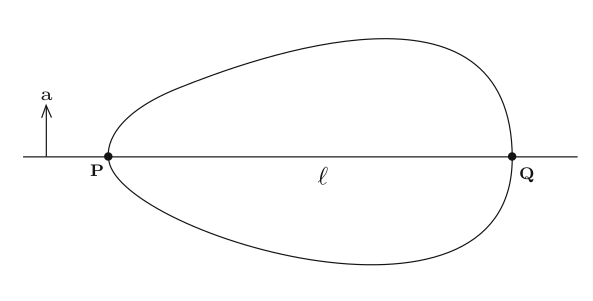
\includegraphics[scale=0.6]{../images/fvt_fig1.png}
		\caption{Reprodução\cite{pressley2001elementary} - Ilustração do vetor $\vec a$}
	\end{figure}
	
	Em um dos lados de $L$, teremos $\gamma\cdotp\vec a>0$, enquanto no outro lado valerá que $ \gamma\cdotp \vec a <0$, a depender do ângulo entre a curva e o vetor $\vec a$ ser agudo ou obtuso. 
	
	Dessa forma a quantidade $\dot \kappa_s(s)(\gamma(s)\cdotp\vec a)$ ou é estritamente positiva, ou é estritamente negativa em todo $s$ exceto $P,Q$.
	
	Sendo assim, a integral
	
	\begin{align}
		\int_0^{\ell}\dot \kappa_s(s)(\gamma(s)\cdotp\vec a)ds\neq0\label{absurd}
	\end{align}

	pois uma propriedade básica de integrais é que se o integrando é não-nulo, a integral é não nula.
	
	Usando o resultado da Propriedade \ref{prop} ($\dot N=-\kappa_s\dot\gamma$), podemos encontrar uma primitiva para a integral acima. Veja que, pela Regra da Cadeia e pela linearidade da derivada, temos que:
	
	$$\dot\kappa_s\gamma = \dot{(\kappa_s\gamma)}-\kappa_s\dot\gamma=\dot{(\kappa_s\gamma)}+\dot N=\dfrac{d}{ds}(\kappa_s\gamma+\dot N)$$
	
	Dado que, fixado $\vec a$ ele é um vetor constante em relação ao parâmetro $s$, então uma primitiva para o integrando acima seria $(\kappa_s\gamma+\dot N)\cdotp \vec a$ que chamaremos de $\lambda(s)$.
	
	Como $\gamma$ é uma curva fechada de comprimento $\ell$ ela é $\ell$-periódica \cite{pressley2001elementary}, ou seja,
	
	$$\gamma(s+\ell)=\gamma(s),$$
	
	para qualquer parâmetro $s$ onde a curva esteja definida.
	
	Diferentiando em relação a $s$, obtemos:
	
	$$T(s+\ell)=T(s)$$
	
	Rotationando os vetores acima por 90 graus antihorários, obtemos:
	
	$$N(s+\ell)=N(s)$$
	
	Assim, $\dot T(s+\ell)=\dot T(s)$, e pela definição de curvatura com sinal, teremos também uma curvatura periódica: 
	$\kappa_s(s+\ell)=\kappa_s(s)$.
	
	Dessa forma, 
	\begin{align*}
		\lambda(s+\ell)&=(\kappa_s(s+\ell)\gamma(s+\ell)+\dot N(s+\ell))\cdotp \vec a\\
		&=(\kappa_s(s)\gamma(s)+\dot N(s))\cdotp \vec a\\
		&=\lambda(s)
	\end{align*}
	
	Então, calculando a integral, cnsiderando a periodicidade de $\lambda$, teríamos:
	
	\begin{align*}
		\int_0^{\ell}\dot \kappa_s(s)(\gamma(s)\cdotp\vec a)ds=\int_0^{\ell}\dfrac{d}{ds}\lambda(s)ds
		=\lambda(\ell)-\lambda(0)=0
	\end{align*}
	
	Absurdo pois em \ref{absurd} concluímos que tal integral era não-nula.
	
	
	\section{Exercícios}
	
	Segue a Resolução dos exercícios da Seção 3.3 de \cite{pressley2001elementary}:
	 
	\begin{enumerate}[3.3.1]
		\item Mostre que a elipse Example $\gamma(s)=(p\cos s,q\sin s)$ com  $p,q\neq0$ é convexa.
		
		
		\textbf{Solução:} Podemos definir o interior da elipse como om conjunto $int(\gamma)=\left\{(x,y)\in\rr;\dfrac{x^2}{p^2}+\dfrac{y^2}{q^2}<1\right\}$
		Sejam $P=(x_p,y_p)$ e $Q=(x_q,y_q)$ pontos interiores da elipse. 
		
		Assim, vale que 
		
		\begin{align*}
			\dfrac{x_p^2}{p^2}+\dfrac{y_p^2}{q^2}<1\text{ e }\dfrac{x_q^2}{p^2}+\dfrac{y_q^2}{q^2}<1
		\end{align*}
	
	Pela Definição de curvas convexas \ref{convexcurve}, precisamos provar que 
	
	$$Pt+(1-t)Q\in int(\gamma),~\forall t\in[0,1],$$
	
	ou seja,
	
	$$(tx_p+(1-t)x_q,ty_p+(1-t)y_q)\in int(\gamma),~\forall t\in[0,1]$$
	
	Basta provar então que 
	
	$$\dfrac{(tx_p+(1-t)x_q)^2}{p^2}+\dfrac{(ty_p+(1-t)y_q)^2}{q^2}<1$$
	
	Fazendo os cálculos:
	
	\begin{align}
		&~~\dfrac{(tx_p+(1-t)x_q)^2}{p^2}+\dfrac{(ty_p+(1-t)y_q)^2}{q^2}\nonumber\\
		&=\dfrac{t^2x_p^2}{p^2}+\dfrac{(1-t)^2x_q^2}{p^2}+\dfrac{t^2y_p^2}{q^2}+\dfrac{(1-t)^2y_q^2}{q^2}+2t(1-t)\left(\dfrac{x_px_q}{p^2}+\dfrac{t_py_q}{q^2}\right)\nonumber\\
		&=t^2\left(\dfrac{x_p^2}{p^2}+\dfrac{y_p^2}{q^2}\right)+(1-t)^2\left(\dfrac{x_p^2}{p^2}+\dfrac{y_p^2}{q^2}\right)+2t(1-t)\left(\dfrac{x_px_q}{p^2}+\dfrac{y_py_q}{q^2}\right)\nonumber\\
		&< t^2+(1-t)^2+2t(1-t)\left(\dfrac{x_px_q}{p^2}+\dfrac{y_py_q}{q^2}\right)\label{ineq}
	\end{align}

	Como $(x_p,y_p)$ e $(x_q,y_q)$ são pontos interiores, podemos usar uma parametrização por coordenadas polares da seguinte forma:
	
	\begin{align*}
		x_p&=pc_1\cos\theta_1\\
		y_p&=qc_1\sin\theta_1\\
		x_q&=pc_2\cos\theta_2\\
		y_q&=qc_2\sin\theta_2\\
		&\text{Para $c_1,c_2\in [0,1)$ e $\theta_1,\theta_2\in\real$}
	\end{align*}

	É facil ver que tais parametrizações satisfazem a condição de pertencer à $int(\gamma)$:
	
	$$\dfrac{x_p^2}{p^2}+\dfrac{y_p^2}{q^2}<\dfrac{p^2\cos^2\theta_1}{p^2}+\dfrac{q^2\sin^2\theta_1}{q^2}=1$$
	
	O mesmo vale para $(x_q,y_q)$.
	Assim, podemos transformar o último termo de \ref{ineq} em:
	
	\begin{align*}
		2t(1-t)\left(\dfrac{x_px_q}{p^2}+\dfrac{y_py_q}{q^2}\right)&=2t(1-t)\left(\dfrac{pc_1\cos\theta_1 pc_2\cos\theta_2}{p^2}+\dfrac{qc_1\sin\theta_1qc_2\sin\theta_2}{q^2}\right)\\
		&=2t(1-t)c_1c_2\left(\cos\theta_1\cos\theta_2+\sin\theta_1\sin\theta_2\right)\\
		&<2t(1-t)\cos(\theta_1-\theta_2)\\
		&<2t(1-t)
	\end{align*}

	Continuando em \ref{ineq}:
	
	\begin{align*}
		&~~~t^2+(1-t)^2+2t(1-t)\left(\dfrac{x_px_q}{p^2}+\dfrac{y_py_q}{q^2}\right)\\
		&<t^2+(1-t)^2+2t(1-t)\\
		&=t^2+1-2t+t^2+2t-2t^2\\
		&=1
	\end{align*}

	o que termina a demonstração.
	\begin{flushright}
	$\blacksquare$
	\end{flushright}

		\item Prove que a limaçon 
		$$\gamma(t)=((1+2\cos t)\cos t,(1+2\cos t)\sin t),t\in\real$$             
		 tem apenas dois vértices.
		 
		 \textbf{Solução: } Vamos analisar os pontos onde derivada da curvatura com sinal é nula.
		 
		 \begin{align*}
		 	\gamma'(t)&=(-(4 \cos t + 1)\sin t, 2\cos2t + \cos t )\\
		 	&=(-2\sin2t-\sin t,2\cos2t+\cos t)\\
		 	\gamma''(t)&=(-\cos t - 4 \cos2t, -\sin t - 4 \sin2t)\\
		 	det[\gamma',\gamma'']&=2\sin2t\sin t+8\sin^22t+\sin^2t+4\sin2t\sin t\\
		 	&~~~-(-2\cos2t\cos t-8\cos^22t-\cos^2t-4\cos2t\cos t)\\
		 	&=8(\sin^22t+\cos^22t)+(\sin^2t+\cos^2t)+6\sin2t\sin t+6\cos2t\cos t\\
		 	&=9+6\cos t(2\sin^2t+\cos^2t-\sin^2t)\\
		 	&=9+6\cos t\\
		 	||\gamma'(t)||&=\sqrt{4\cos t+5}
      \end{align*}
  
  Assim:
  
  \begin{align*}
  	\kappa_s(t)&=\dfrac{9+6\cos t}{(4\cos t+5)^{3/2}}
  	\end{align*}
  
  Derivando, temos:
  
  \begin{align*}
  	\kappa_s'(t)&=\dfrac{(4\cos t+5)^{3/2}[-6\sin t]-(9+6\cos t)[-6\sin t(4\cos t+5)^{1/2}]}{(4\cos t+5)^3}
  \end{align*}

	Como cosseno é limitado entre -1 e 1 a expressão $4\cos t+5$ nunca se anula, logo podemos dividir numerador e denominador acima por $(4\cos t+5)^{1/2}$, e obtemos:
	
	\begin{align*}
		\kappa_s'(t)&=\dfrac{-(4\cos t+5)6\sin t+6\sin t(9+6\cos t)}{(4\cos t+5)^{5/2}}\\
		&=\dfrac{12\cos t\sin t+24\sin t}{(4\cos t+5)^{5/2}}\\
		&=\dfrac{12\sin t(2+\cos t)}{(4\cos t+5)^{5/2}}
	\end{align*}

	Como $(2+\cos t)>0~\forall t \in \real$, a expressão acima só é zero quando $12\sin t=0$, ou seja, considerando apenas a "primeira volta"\footnote{A limaçon é $2\pi$ periódica.} da curva, os pontos $t=0$ e $t=\pi$. Logo, a curva tem apenas dois vértices.
	
	Isso não é um contraexemplo para o teorema, pois a limaçon não é uma curva de Jordan, pois possui um auto-interseção, fazendo com que seu traço não defina apenas duas componentes conexas.
		 
		 \item Prove que a curva plana $\gamma$ possui um vértice em $t=t_0$ se, e somente se, a evoluta $\epsilon$ de $\gamma$ tem um ponto singular em $t=t_0$.
		 
		 \textbf{Solução:} Supondo $\gamma$ \textit{unit-speed}, usando $\epsilon(s)=\gamma(s)+\dfrac{1}{\kappa_s(s)}N(s)$, e diferenciando $\epsilon$ temos:
		 \begin{align*}
		 	\dot{\epsilon}(s)&=\dot \gamma (s)+\dfrac{\kappa_s\dot N(s)-\dot\kappa_s(s)N(s)}{\kappa_s(s)}\\
		 	&\text{Pela Propriedade \ref{prop}, segue que:}\\
		 	&=\dot\gamma(s)+\dfrac{-\kappa_s^2\dot\gamma(s)-\dot\kappa_s(s)N(s)}{\kappa_s^2(s)}\\
		 	&=\dfrac{\cancel{\kappa_s^2\dot\gamma(s)}-\cancel{\kappa_s^2\dot\gamma(s)}-\dot\kappa_s(s)N(s)}{\kappa_s^2(s)}\\
		 	&=\dfrac{-\dot\kappa_s(s)N(s)}{\kappa_s^2(s)}
		 \end{align*}

	Note que como $\dfrac{N(s)}{\kappa_s^2(s)}$ não se anula, então $\dot\epsilon(s)$ será nula se, e somente se $\dot\kappa_s(s)=0$.
	
	Logo, $\gamma$ possui um vértice em $t_0$, se, e somente se, $\dot\epsilon(t_0)=0$, ou seja a evoluta $\epsilon$ de $\gamma$ tem um ponto singular em $t_0$.
		 
	\end{enumerate}
	
	\section{Exemplo Geogebra}
	\href{https://www.geogebra.org/calculator/kzzrgkxp}{Neste link} há um exemplo interativo mostrando uma elipse $\gamma(t)=(a\cos t,b\sin t)$. Com passos simples de cálculo é possível mostrar que a derivada da curvatura de $\gamma$ é:
	
	$$\dfrac{d\kappa_s}{dt}=\dfrac{3ab(b^2-a^2)\sin t\cos t}{(a^2\sin^2t+b^2\cos^2t)^{5/2}}$$
	
	O arquivo contém um controle deslizante que controla a posição de um ponto $A$ sobre a curva. Pela fórmula acima, se $b\neq a$, a derivada é nula em $t=0,\frac{\pi}2,\pi,\frac{3\pi}2$. Ao fazer o controle deslisante passar por esses valores é possível ver a troca de sinal na variável dk, definina no GeoGebra como a fórmula acima. Tem-se assim, exatamente 4 vértices.
	
	No caso $b=a$, temos uma circunferência, de curvatura constante, cuja derivada é nula em todos os pontos, ou seja, a circunferência tem infinitos vértices.
	
	\newpage
	\addcontentsline{toc}{section}{Referências}
%	\bibliography{refs}
	\printbibliography
\end{document}